\section{PROCEDIMIENTO} 

\begin{itemize}
\subsection{Instalacion de Docker}
	
	\item Instalar Docker desde la siguiente direccion :
	https://docs.docker.com/docker-for-windows/install/
	\begin{figure}[htb]
	\begin{center}
	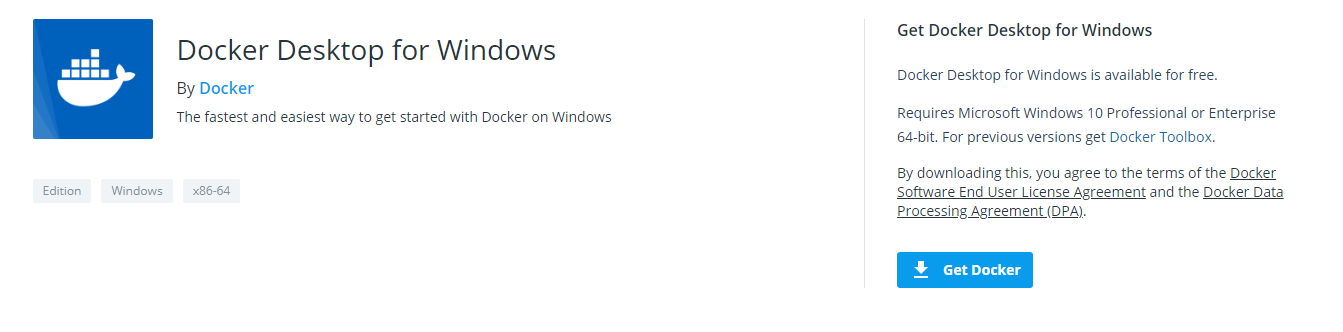
\includegraphics[width=18cm, height=8cm]{./Imagenes/docker}
	\end{center}
	\end{figure}\\
	
	\item Seguir el proceso de Instalacion :\\
	\begin{figure}[htb]
	\begin{center}
	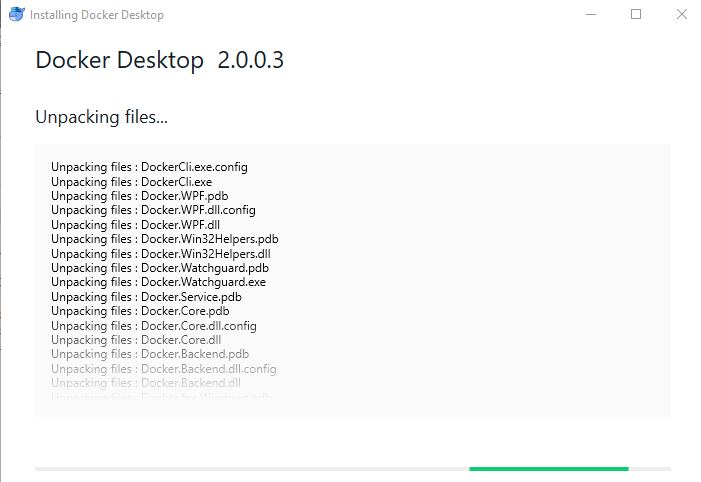
\includegraphics[width=18cm, height=8cm]{./Imagenes/dockerinst}
	\end{center}
	\end{figure}\\
	
	\item Reiniciar la PC :\\
	\begin{figure}[htb]
	\begin{center}
	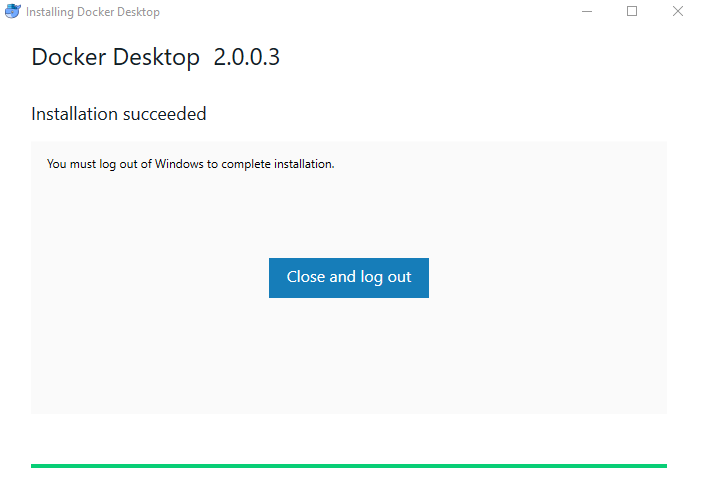
\includegraphics[width=18cm, height=8cm]{./Imagenes/dockerre}
	\end{center}
	\end{figure}
	
	\item Comprobar que docker ha sido instalado correctamente:\\	
	\begin{figure}[htb]
	\begin{center}
	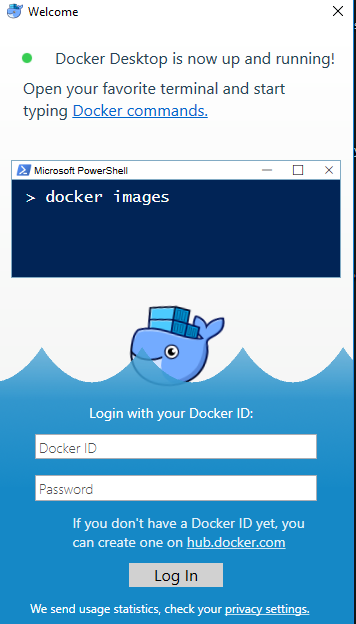
\includegraphics[width=7cm, height=8cm]{./Imagenes/dockerrun}
	\end{center}
	\end{figure}\\\\\\\\		
		
\subsection{Iniciando en Docker}
	
	\item Logearse con su cuenta y contraseña Respectiva:\\
			
	\begin{figure}[htb]
	\begin{center}
	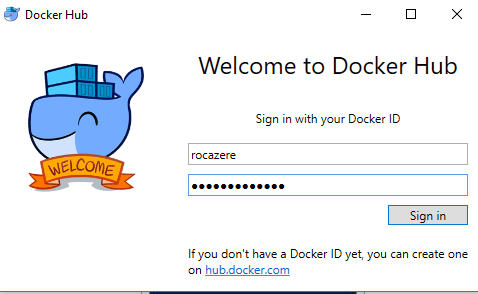
\includegraphics[width=8cm, height=6cm]{./Imagenes/dockerlogin}
	\end{center}
	\end{figure}
	
	\item Iniciar la consola PowerShell de Windows:\\
	
	\begin{figure}[htb]
	\begin{center}
	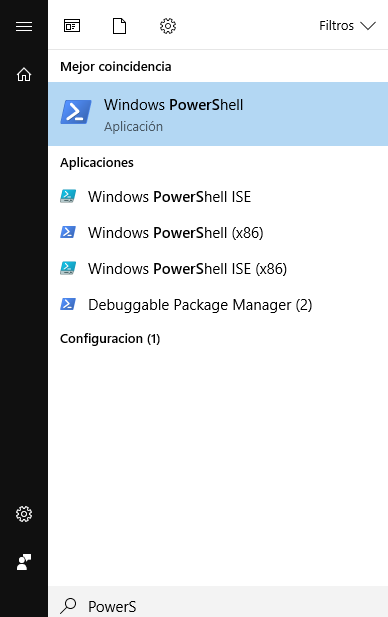
\includegraphics[width=8cm, height=10cm]{./Imagenes/powershell}
	\end{center}
	\end{figure}
	\clearpage
	
	\subsection{Creando un contenedor Miscrosoft SQL para Linux}
	
	\item Como primer comando usaremos:  "docker version" para ver la    version de docker que acabamos de instalar:\\
	
	
	\begin{figure}[htb]
	\begin{center}
	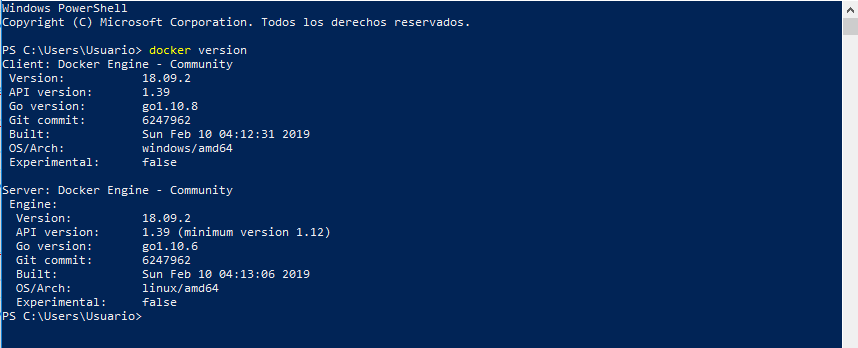
\includegraphics[width=16cm, height=8cm]{./Imagenes/dockerversion}
	\end{center}
	\end{figure}
	
	\item Ahora crearemos un contenedor con Microsoft SQL server para Linux, para esto usaremos primero el comando "docker search mssql":\\
	
	
	\begin{figure}[htb]
	\begin{center}
	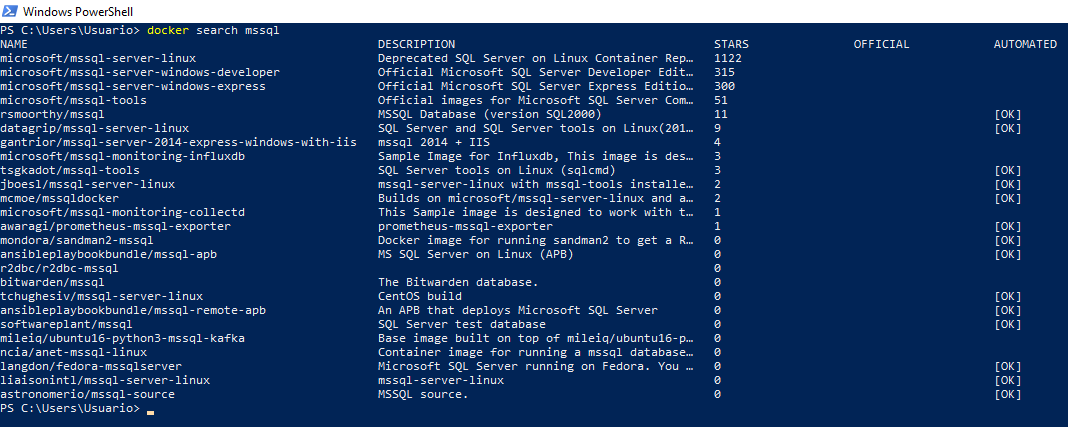
\includegraphics[width=16cm, height=8cm]{./Imagenes/dockersearch}
	\end{center}
	\end{figure}
	\clearpage
	
	\item Luego descargaremos la imagen del contenedor de Microsoft SQL en un servidor Linux con el siguiente comando "docker pull microsoft/mssql-server-linux":\\
	
	
	\begin{figure}[htb]
	\begin{center}
	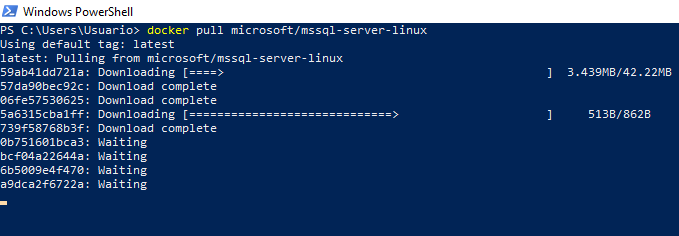
\includegraphics[width=16cm, height=8cm]{./Imagenes/dockerdownload}
	\end{center}
	\end{figure}
	
	\item esperar un determinado tiempo a que descargue todo:\\
	
	
	\begin{figure}[htb]
	\begin{center}
	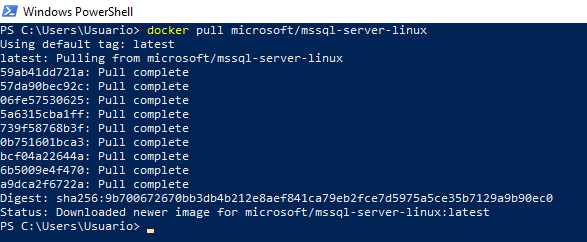
\includegraphics[width=16cm, height=8cm]{./Imagenes/dockerdownloaded}
	\end{center}
	\end{figure}
	\clearpage
	
	\item Para ver la imagen que acabamos de descargar, usaremos el siguiente comando: "docker images":\\
	
	
	\begin{figure}[htb]
	\begin{center}
	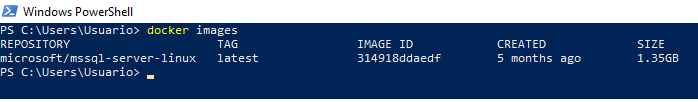
\includegraphics[width=16cm, height=3cm]{./Imagenes/dockerimages}
	\end{center}
	\end{figure}
	
	\item Ahora crearemos credenciales los cuales usaremos mas adelante para autenticar nuestra entrada a SQL server, usaremos el siguiente comando: 
	
	
	\begin{figure}[htb]
	\begin{center}
	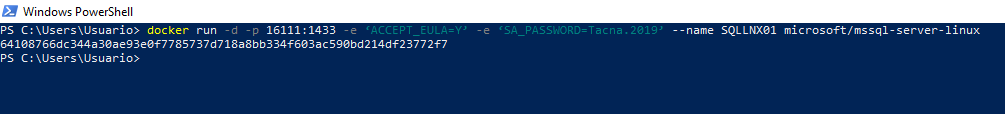
\includegraphics[width=16cm, height=3cm]{./Imagenes/dockercred}
	\end{center}
	\end{figure}
	
	\item Accedemos a dar los permisos para el firewall de Windows
	
	\begin{figure}[htb]
	\begin{center}
	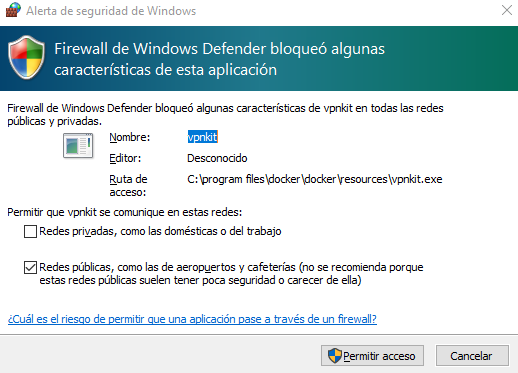
\includegraphics[width=10cm, height=9cm]{./Imagenes/firewall}
	\end{center}
	\end{figure}
	
	\item Verificamos la correcta ejecucion del contenedor con el comando "docker ps":\\
	
	\begin{figure}[htb]
	\begin{center}
	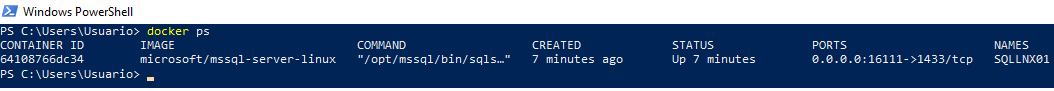
\includegraphics[width=16cm, height=2cm]{./Imagenes/dockerps}
	\end{center}
	\end{figure}
	
	\item Accedemos a Sql server con los siguientes credenciales:\\
	
	\begin{figure}[htb]
	\begin{center}
	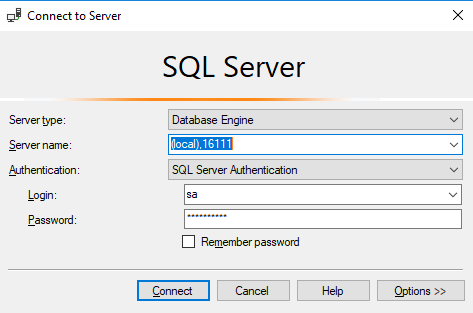
\includegraphics[width=10cm, height=9cm]{./Imagenes/sql}
	\end{center}
	\end{figure}
	
	\item En sql iniciairemos un nuevo query para hacer una consulta sobre la version:\\
	
	\begin{figure}[htb]
	\begin{center}
	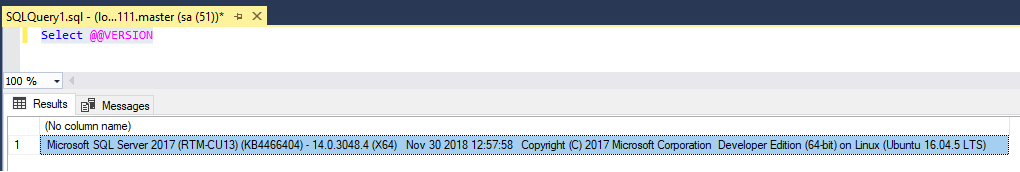
\includegraphics[width=18cm, height=4cm]{./Imagenes/sqlconsulta}
	\end{center}
	\end{figure}
	\clearpage
	\item Ahora cerraremos Sql server y procederemos a eliminar el contenedor creado con el siguiente comando: "docker rm -f SQLLNX01" y despues comprobaremos que este ha sido eliminado:\\
	
	\begin{figure}[htb]
	\begin{center}
	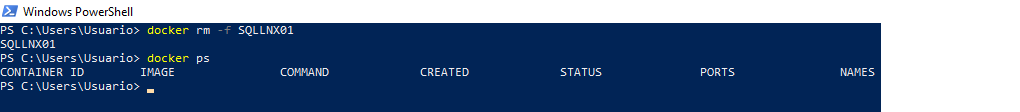
\includegraphics[width=21cm, height=4cm]{./Imagenes/dockerele}
	\end{center}
	\end{figure}
	\clearpage
	\subsection{Adicionando una Persistencia}
	
	\item Crearemos un nuevo contenedor, verificaremos que este ha sido creado correctamente y luego iniciaremos sesion con los respectivos credenciales:\\
	
	
	\begin{figure}[htb]
	\begin{center}
	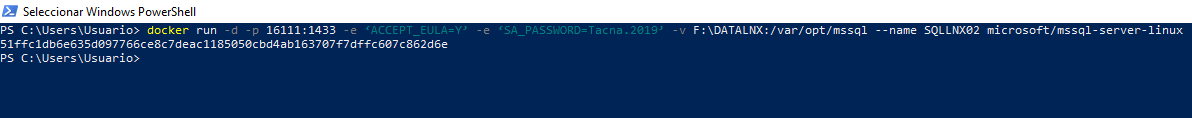
\includegraphics[width=16cm, height=4cm]{./Imagenes/daltan}
	\end{center}
	\end{figure}
	
	\begin{figure}[htb]
	\begin{center}
	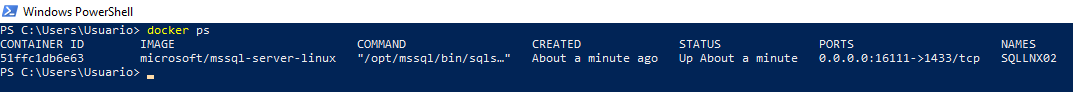
\includegraphics[width=16cm, height=4cm]{./Imagenes/dockerps2}
	\end{center}
	\end{figure}
	
	
	\begin{figure}[htb]
	\begin{center}
	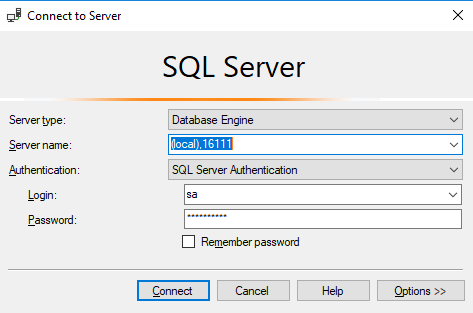
\includegraphics[width=9cm, height=7cm]{./Imagenes/sql}
	\end{center}
	\end{figure}
	\clearpage
	
	\item Ahora crearemos una base de datos con el siguiente Script:\\
	
	\begin{figure}[htb]
	\begin{center}
	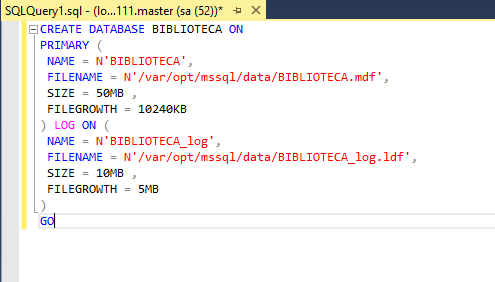
\includegraphics[width=19cm, height=8cm]{./Imagenes/script}
	\end{center}
	\end{figure}
	
	\item Verificaremos que la carpeta DATALNX contenga esta base de datos:\\
	
	\begin{figure}[htb]
	\begin{center}
	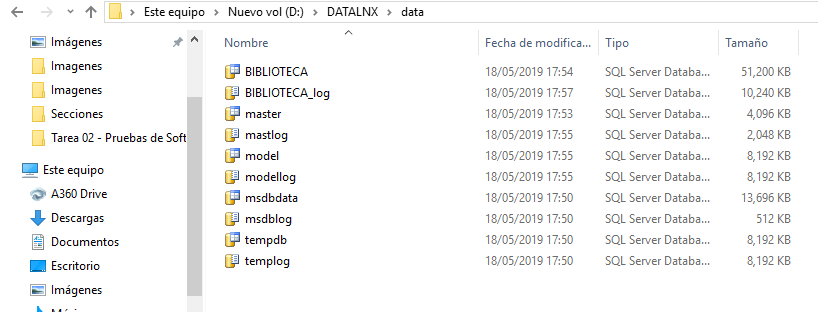
\includegraphics[width=19cm, height=8cm]{./Imagenes/datal}
	\end{center}
	\end{figure}
	
	\item Por ultimo eliminaremos este contenedor.\\
	\clearpage
	
	
	\subsection{Creando un contenedor con Microsoft SQL para Windows}
	
	\item En la parte inferior derecha encontraremos el icono de Docker el cual al hacerle click derecho, abrira un menu desplegable en el que seleccionaremos Switch to windows containers... y esperaremos a que docker se reinicie:\\
	
	\begin{figure}[htb]
	\begin{center}
	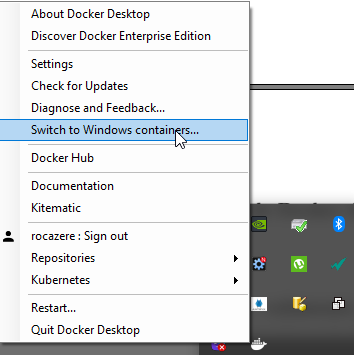
\includegraphics[width=17cm, height=7cm]{./Imagenes/winco}
	\end{center}
	\end{figure}
	
	\item Ahora en la ventana de PowerShell usaremos los siguientes comandos::\\
	
	
	\begin{figure}[htb]
	\begin{center}
	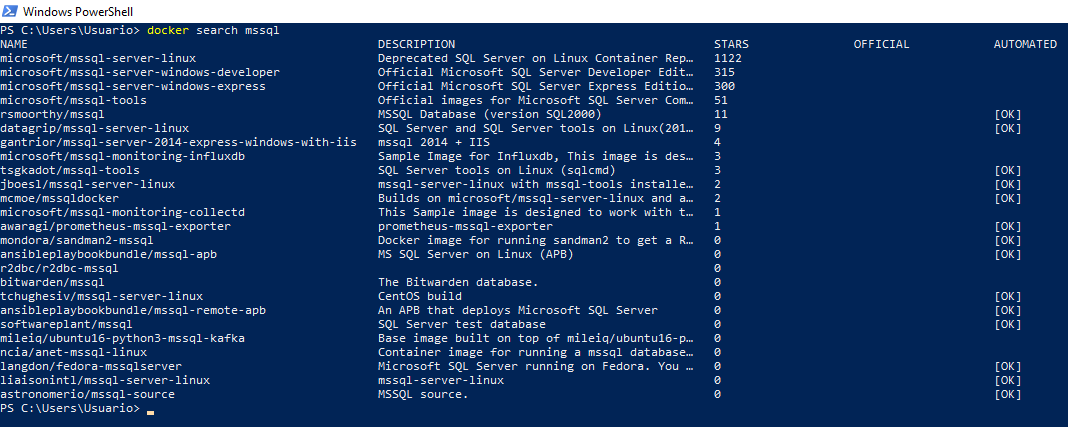
\includegraphics[width=17cm, height=7cm]{./Imagenes/dockersearch}
	\end{center}
	\end{figure}
	\clearpage
	\item Instalaremos el contenedor de Microsoft sql para un servidor Windows:\\
			
	\begin{figure}[htb]
	\begin{center}
	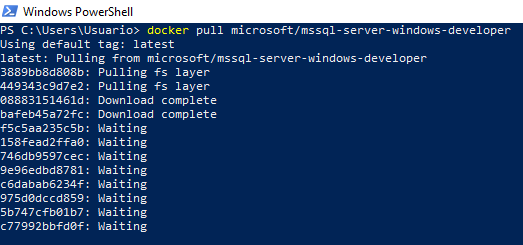
\includegraphics[width=17cm, height=7cm]{./Imagenes/windows}
	\end{center}
	\end{figure}
	
	\item Comprobaremos la correcta instalacion del contenedor con el comando "docker images":\\
	
	\begin{figure}[htb]
	\begin{center}
	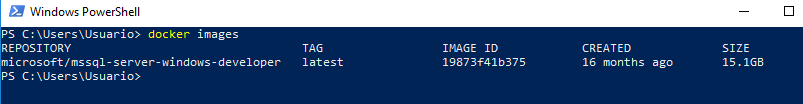
\includegraphics[width=15cm, height=5cm]{./Imagenes/windowsimages}
	\end{center}
	\end{figure}
	\clearpage
	
	\item Crearemos nuevos credenciales para este nuevo contenedor Sql para servidores windows:\\
	
	\begin{figure}[htb]
	\begin{center}
	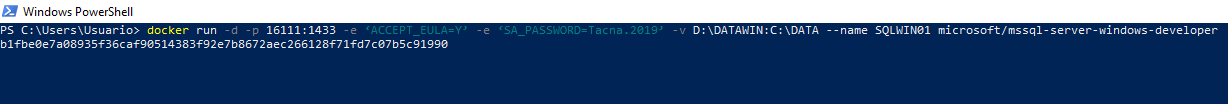
\includegraphics[width=20cm, height=3cm]{./Imagenes/credenciales}
	\end{center}
	\end{figure}
	
	\item Iniciaremos sesion en Sql con las credenciales que hemos creado:\\
	
	\begin{figure}[htb]
	\begin{center}
	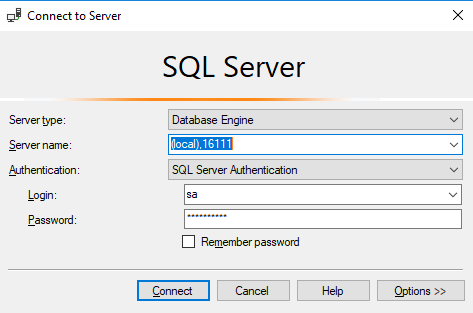
\includegraphics[width=10cm, height=9cm]{./Imagenes/sql}
	\end{center}
	\end{figure}
	\clearpage
	\item revisamos la version: 	
	
	\begin{figure}[htb]
	\begin{center}
	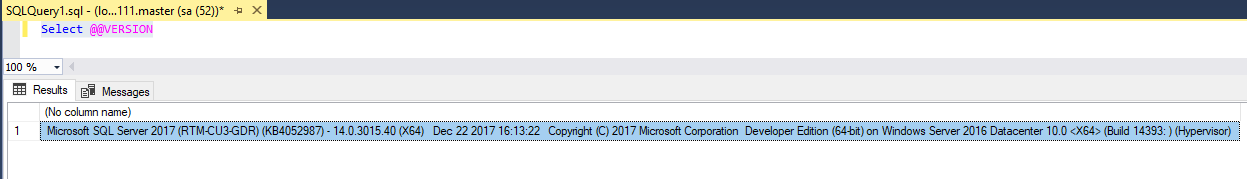
\includegraphics[width=18cm, height=4cm]{./Imagenes/sqlwindows}
	\end{center}
	\end{figure}
	
	\item Mediante el siguiente scrip generaremos una base de datos de prueba:\\
	
	\begin{figure}[htb]
	\begin{center}
	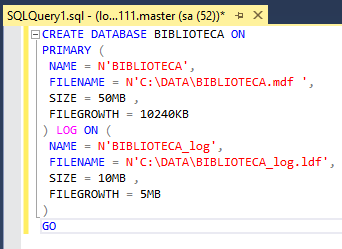
\includegraphics[width=10cm, height=8cm]{./Imagenes/scrip}
	\end{center}
	\end{figure}
	\clearpage
	\item Comprobaremos que la base de datos ha sido creada:\\
	
	\begin{figure}[htb]
	\begin{center}
	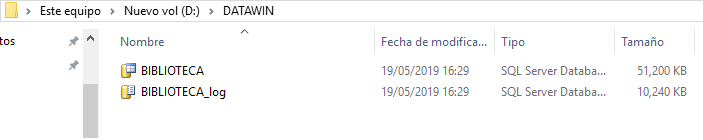
\includegraphics[width=16cm, height=4cm]{./Imagenes/datawin}
	\end{center}
	\end{figure}
	
	\item Finalmente procederemos con la eliminacion del conteneder y verificaremos que esta ha sido eliminada:\\
	
	\begin{figure}[htb]
	\begin{center}
	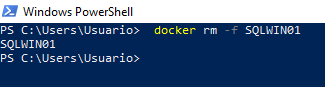
\includegraphics[width=10cm, height=5cm]{./Imagenes/dockerrm}
	\end{center}
	\end{figure}
	
	\begin{figure}[htb]
	\begin{center}
	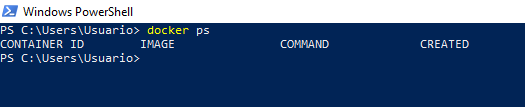
\includegraphics[width=12cm, height=3cm]{./Imagenes/dockerpsss}
	\end{center}
	\end{figure}
	\clearpage
	
	\subsection{Actividades Encargadas}
	
	\subsubsection{¿Con qué comando(s) exportaría la imagen de Docker de Microsoft SQL Server a otra PC o servidor?}
	
	\item uno de los comandos usados para exportar un contendor seria:
	
		\begin{figure}[htb]
	\begin{center}
	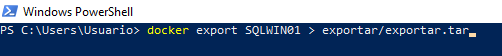
\includegraphics[width=12cm, height=3cm]{./Imagenes/tar}
	\end{center}
	\end{figure}
	
	Podemos observar que hemos guardar un archivo .tar en nuestra carpeta usuarios. Luego esto podra ser transportando ha otra maquina ya sea windows o linux.
		\begin{figure}[htb]
	\begin{center}
	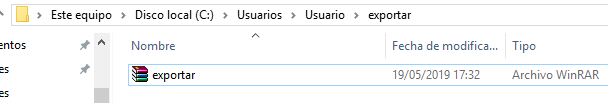
\includegraphics[width=12cm, height=3cm]{./Imagenes/tar2}
	\end{center}
	\end{figure}
	\clearpage
	
	
	
	\subsubsection{¿Con qué comando(s) podría generar dos volúmenes para un contenedor?}
	
	\item Los volumenes pueden ser gestionados con el siguiente comando:
	
	\begin{figure}[htb]
	\begin{center}
	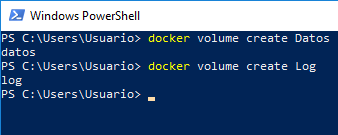
\includegraphics[width=12cm, height=3cm]{./Imagenes/volumenes}
	\end{center}
	\end{figure}
	
	\item Con el siguiente comando, podremos ver donde estos han sido creados:
	
	
	\begin{figure}[htb]
	\begin{center}
	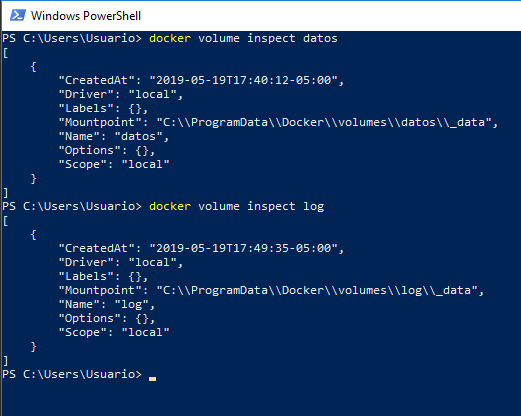
\includegraphics[width=10cm, height=9cm]{./Imagenes/volumenes2}
	\end{center}
	\end{figure}
	
	Ahora podremos usar estos volumens creado para crear nuestros archivos .mdf y .log en sus repectivos directorios.
	\clearpage
	
	
	
	\subsubsection{Genere un nuevo contenedor con las siguientes caracteristicas:}
	
	\item El Script es:
	
	\begin{figure}[htb]
	\begin{center}
	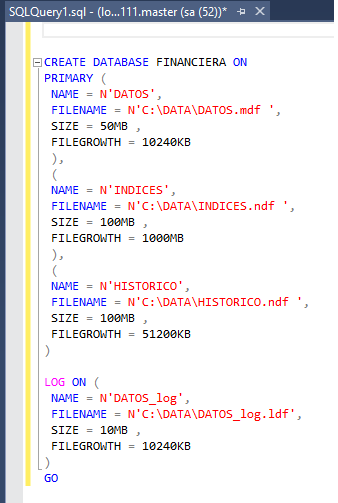
\includegraphics[width=10cm, height=9cm]{./Imagenes/scriptq}
	\end{center}
	\end{figure}
	
	\item Verificamos que haya sido creado correctamente:
	
	\begin{figure}[htb]
	\begin{center}
	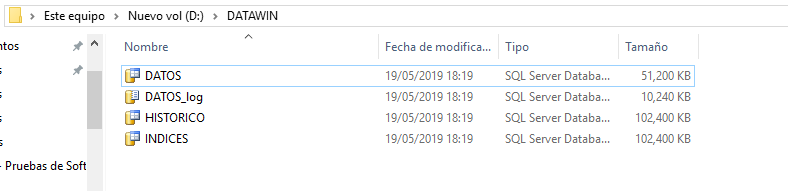
\includegraphics[width=10cm, height=6cm]{./Imagenes/scriptq2}
	\end{center}
	\end{figure}
	
	
	
	

\end{itemize}